\documentclass[journal]{IEEEtran}
\usepackage[a5paper, margin=10mm]{geometry}
%\usepackage{lmodern} % Ensure lmodern is loaded for pdflatex
\usepackage{tfrupee} % Include tfrupee package

%iffalse
\let\negmedspace\undefined
\let\negthickspace\undefined
\usepackage{gvv-book}
\usepackage{gvv}
\usepackage{cite}
\usepackage{amsmath,amssymb,amsfonts,amsthm}
\usepackage{algorithmic}
\usepackage{graphicx}
\usepackage{textcomp}
\usepackage{xcolor}
\usepackage{txfonts}
\usepackage{listings}
\usepackage{enumitem}
\usepackage{mathtools}
\usepackage{gensymb}
\usepackage{comment}
\usepackage[breaklinks=true]{hyperref}
\usepackage{tkz-euclide} 
\usepackage{listings}                                        
%\def\inputGnumericTable{}                                 
\usepackage[latin1]{inputenc}                                
\usepackage{color}                                            
\usepackage{array}                                            
\usepackage{longtable}                                       
\usepackage{calc}                                             
\usepackage{multirow}                                         
\usepackage{hhline}                                           
\usepackage{ifthen}                                           
\usepackage{lscape}
\usepackage{tabularx}
\usepackage{array}
\usepackage{float}
\usepackage{multicol}

\newcommand{\BEQA}{\begin{eqnarray}}
\newcommand{\EEQA}{\end{eqnarray}}
%\newcommand{\define}{\stackrel{\triangle}{=}}

\setlength{\headheight}{1cm} % Set the height of the header box
\setlength{\headsep}{0mm}     % Set the distance between the header box and the top of the text


%\usepackage[a5paper, top=10mm, bottom=10mm, left=10mm, right=10mm]{geometry}


\setlength{\intextsep}{10pt} % Space between text and floats

% Marks the beginning of the document
\begin{document}
\onecolumn
\bibliographystyle{IEEEtran}
\vspace{3cm}

%\renewcommand{\theequation}{\theenumi}
\numberwithin{equation}{enumi}
\numberwithin{figure}{enumi}
\renewcommand{\thefigure}{\theenumi}
\renewcommand{\thetable}{\theenumi}

\title{1-1.9-4}
\author{ai24btech11030 - Shiven Bajpai}
\maketitle

\renewcommand{\thefigure}{\theenumi}
\renewcommand{\thetable}{\theenumi}

\textbf{Question: } If $\vert\vert\vec{a}\vert\vert = 4$ and $-3 \leq \lambda \leq 2$, then $\vert\vert \lambda \vec{a}\vert\vert$ lies in

\begin{enumerate}
    \item \sbrak{0, 12}
    \item \sbrak{2, 3}
    \item \sbrak{8, 12}
    \item \sbrak{-12, 8}
\end{enumerate}

\textbf{Solution: } 1) \sbrak{0, 12}

\begin{align*}
    \vert\vert\vec{a}\vert\vert &= \sqrt{\vec{a}\vec{a}^\text{T}}\\
    \vert\vert\lambda\vec{a}\vert\vert &= \sqrt{\brak{\lambda \vec{a}}\brak{\lambda \vec{a}}^\text{T}}\\
    &= \sqrt{\lambda^2 \vec{a}\vec{a}^\text{T}}\\
    &= \vert\lambda\vert \sqrt{\vec{a}\vec{a}^\text{T}}\\
    \\
    \vert\vert\lambda\vec{a}\vert\vert &= \vert\lambda\vert \, \vert\vert\vec{a}\vert\vert
\end{align*}

Now, since

\begin{align*}
    -3 \leq& \; \lambda \leq 2\\
    0 \leq& \; \vert\lambda\vert \leq 3\\
    0\vert\vert\vec{a}\vert\vert \leq&\, \vert\lambda\vert\,\vert\vert\vec{a}\vert\vert \leq 3\vert\vert\vec{a}\vert\vert\\
    0 \leq&\, \vert\vert\lambda\vec{a}\vert\vert \leq 12\\
\end{align*}



\begin{figure}[H]
	\centering
	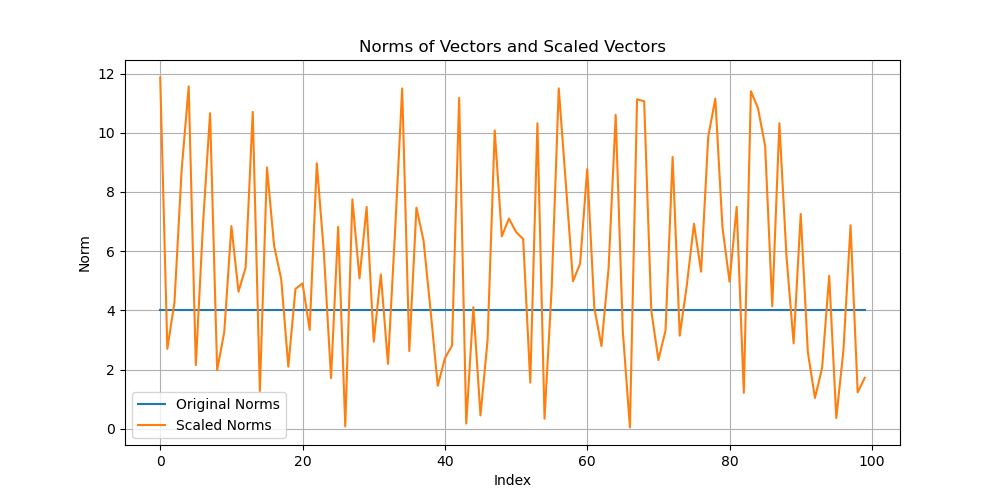
\includegraphics[width=0.75\columnwidth]{Figures/Figure.png}
	\caption{Plot of norms of 100 random vectors, multiplied by random $\lambda$ for each vector, One can see that norm of $\lambda\vec{a}$ is in range \sbrak{0 ,12}}
	\label{fig}
\end{figure}

Code for this plot can be found at:
\begin{lstlisting}
    Codes/main.py
    Codes/main.c
\end{lstlisting}

\end{document}
